\documentclass[11pt,a4paper]{article}
\usepackage[utf8]{inputenc}
\usepackage[T1]{fontenc}
\usepackage[margin=2.3cm]{geometry}
\usepackage{graphicx}
\usepackage{booktabs}
\usepackage{cite}
\usepackage{url}
\usepackage{hyperref}
\usepackage{tikz}
\usetikzlibrary{arrows.meta,positioning,calc}
\usepackage{caption}
\usepackage{subcaption}
\usepackage{microtype}
\usepackage{placeins}
\usepackage{float}

\hypersetup{
  colorlinks=true,
  linkcolor=blue!60!black,
  urlcolor=blue!70!black,
  citecolor=blue!60!black,
}
% Break long Hugging Face model ids at hyphens/underscores (avoids margin overflow)
\makeatletter
\g@addto@macro\UrlBreaks{\do\-\do\_}
\makeatother

\graphicspath{{../screenshots/}}

\title{French Insurance Customer Reviews:\\
NLP Analysis, Thematic Classification, and Interactive Application}
\author{Gabriel Sutlan --- NLP Project 2}
\date{}

\begin{document}
\maketitle

\begin{center}
  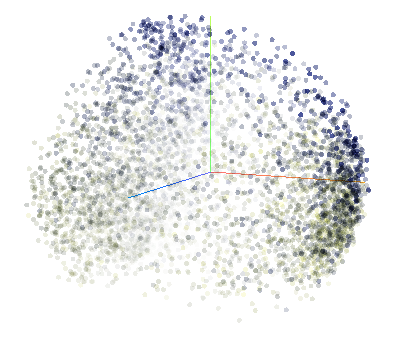
\includegraphics[width=\textwidth]{mainImage.png}\\[0.35em]
  {\small\textit{Cover visual: three-dimensional Word2Vec projection of review tokens, coloured by average rating (\texttt{viridis})---not counted in the figure list.}}
\end{center}
\vspace{0.6em}

\begin{abstract}
This report describes an end-to-end natural language processing project on French insurance customer reviews: data preparation and exploratory analysis, distributional and neural representations (Word2Vec, FastText, LDA), supervised thematic classification (TF-IDF with logistic regression and fine-tuned DistilBERT), and a Streamlit application combining summarization, sentiment analysis, retrieval-augmented question answering, and a multi-stage similar-review search pipeline.
\end{abstract}

\section{Dataset and objectives}
The corpus consists of French reviews with metadata such as insurer (\texttt{assureur}), rating (\texttt{note}), product type, and publication dates. The analytical goal is to surface recurring themes (claims, customer service, pricing, reimbursements, etc.), compare classical and transformer-based classifiers, and expose the results through an interactive tool suitable for qualitative exploration.

\section{``Cleaned'' data and time-saving scale variables}
The exported ``cleaned'' table is the result of a pragmatic pipeline rather than a full pass over every row of the original CSV. To respect time constraints during development, the notebook applies \textbf{scale factors} to expensive steps: spell correction uses a random fraction \texttt{SPELL\_SCALE = 0.01} (one percent of rows), and English translation uses \texttt{TRANSLATE\_SCALE = 0.005}. French abstractive summaries with BARThez use \texttt{RESUME\_FRAC = 0.02}. Setting these parameters to \texttt{1.0} would process the entire dataset; in a real deployment one would typically validate the stack on a subset, then switch the scales to full coverage for the final artifact. The Streamlit preprocessing path (\texttt{review\_preprocess.py}) mirrors the core text normalization used for thematic modeling (lowercasing, punctuation removal, NLTK tokenization, French stopwords, \texttt{simplemma} lemmatization) and does not depend on those partial corrections for inference.

\section{Preprocessing for modeling}
Token-level preprocessing follows a fixed recipe aligned with the notebook: apostrophes are normalized, punctuation is stripped, tokens are filtered by length and digits, and lemmas are produced with \texttt{simplemma} for French. Stopwords come from the notebook artifact when available, otherwise NLTK French stopwords. This design favors a compact vocabulary for bag-of-words and embedding training while preserving insurance-related terms that carry sentiment and topic signal.

\textbf{Lemmatization vs.\ stemming.} French is morphologically rich; rule-based stemmers (e.g.\ Snowball) often truncate surface forms to arbitrary stems that are neither valid words nor unique lemmas, which can merge unrelated senses or split related ones. Lemmatization maps inflected tokens to a canonical dictionary form using linguistic knowledge, yielding tokens that remain human-readable and stable across conjugations and agreements (\textit{assur\'e}, \textit{assur\'es}, \textit{assurer} $\rightarrow$ a single lemma where appropriate). That choice improves interpretability of LDA topics, TF-IDF features, and Word2Vec neighborhoods, and reduces spurious vocabulary fragmentation compared with aggressive stemming.

\section{Exploratory analysis and n-grams}
Unigrams, bigrams, and trigrams were compared before and after cleaning using \texttt{CountVectorizer} with \texttt{max\_features=50} on a sample of 5{,}000 raw texts versus all processed texts. The cap at 50 keeps only the most frequent n-grams for each order so the bar charts stay legible; this step is purely exploratory visualization and is unrelated to the much larger vocabularies used later for supervised models (e.g.\ TF-IDF with thousands of features). Figures~\ref{fig:ngrams} and~\ref{fig:yearly} are placed immediately below; they belong to this section and precede the embedding analysis.

\begin{figure}[H]
  \centering
  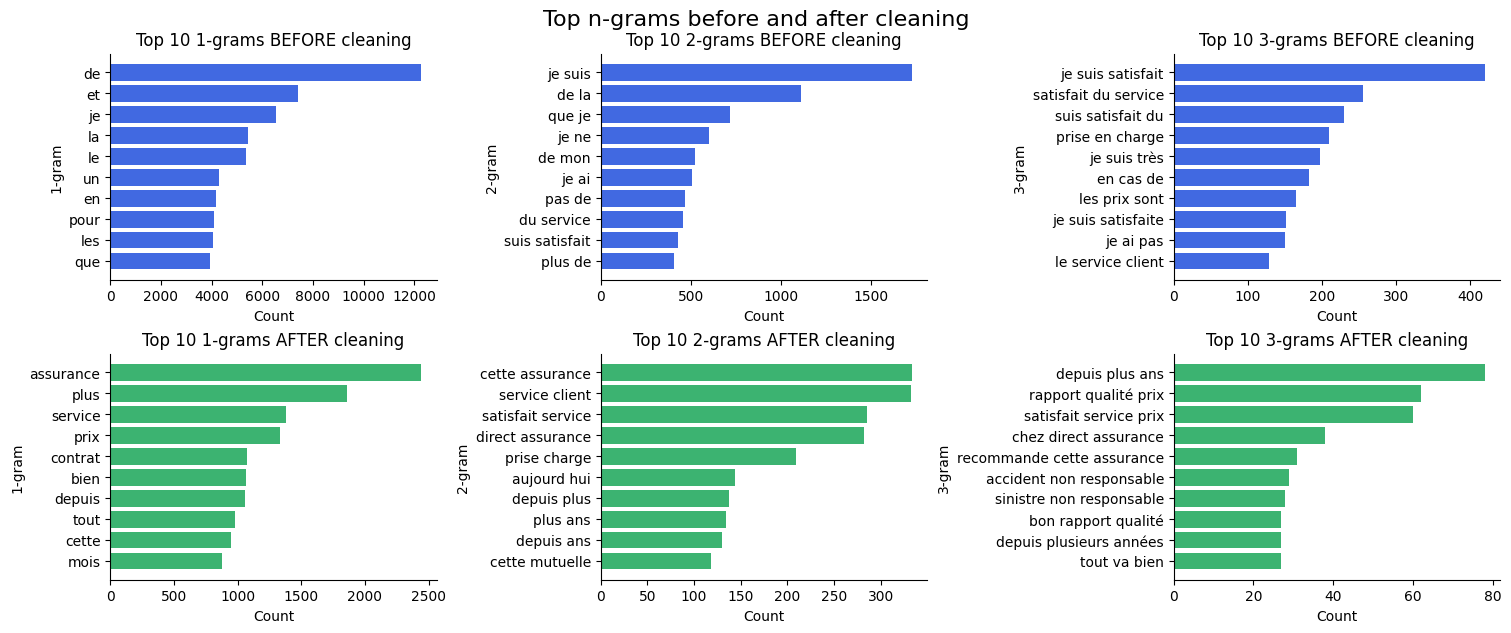
\includegraphics[width=0.92\linewidth]{N-grams.png}
  \caption{N-gram frequency comparison (before vs.\ after preprocessing) for unigrams, bigrams, and trigrams.}
  \label{fig:ngrams}
\end{figure}

\begin{figure}[H]
  \centering
  \begin{subfigure}{0.48\textwidth}
    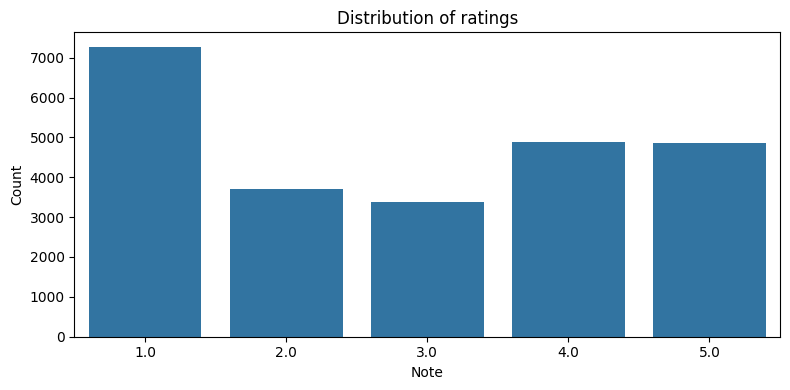
\includegraphics[width=\linewidth]{Distribution_of_ratings.png}
    \caption{Rating distribution (\texttt{countplot} on \texttt{note}).}
  \end{subfigure}\hfill
  \begin{subfigure}{0.48\textwidth}
    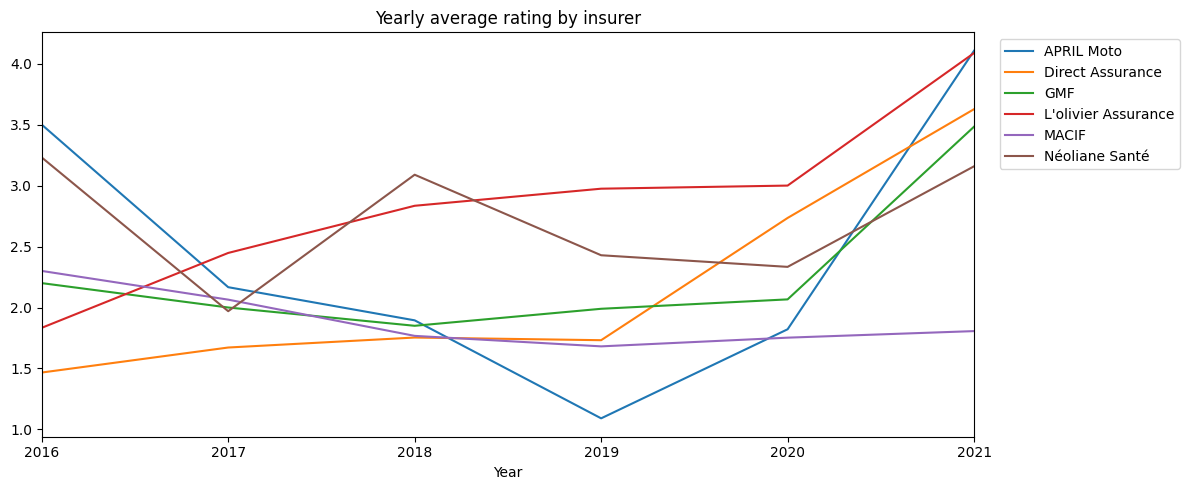
\includegraphics[width=\linewidth]{Yearly_average_rating_by_insurer.png}
    \caption{Yearly mean \texttt{note} by insurer (top insurers by volume).}
  \end{subfigure}
  \caption{Descriptive views of the review scores (notebook EDA).}
  \label{fig:yearly}
\end{figure}

\textbf{Reading the figures.} Figure~\ref{fig:ngrams} echoes the notebook comparison: \emph{before} cleaning, the top token barcodes are noisier---punctuation-driven fragments, duplicated morphological variants, and very generic French forms still compete for mass. \emph{After} lemmatization and filtering, mass shifts toward lemmas that carry insurance semantics (\textit{contrat}, \textit{sinistre}, \textit{remboursement}, \textit{service}, etc.), so each row of panels is easier to read as a sanity check that preprocessing aligns the vocabulary with downstream topic and embedding models. The left panel of Figure~\ref{fig:yearly} shows that star ratings are \emph{not} uniform: low and high scores are heavily represented relative to the mid-scale, with an overall mean close to 2.8--2.9 on the cleaned table (as printed in the notebook after row filtering), so any classifier or sampler must tolerate class imbalance. The right panel aggregates mean ratings by year for the busiest insurers; trajectories differ across companies and years, which cautions against treating the corpus as a single homogeneous stream when interpreting sentiment or themes.

\FloatBarrier

\section{Word2Vec and FastText embeddings}
\textbf{Word2Vec} was trained with Gensim on lemmatized review tokens: \texttt{vector\_size=200}, \texttt{window=5}, \texttt{min\_count=7}, \texttt{workers=1}, \texttt{seed=42} (these choices are results of empirical trials). The dimension and context window follow common defaults for medium-sized corpora; \texttt{min\_count} suppresses rare tokens that inflate noise. Technical reference~\cite{ref:gensim-w2v}. Two-dimensional PCA projections color words by average rating help interpret semantic neighborhoods (Figure~\ref{fig:w2vft}).

\textbf{FastText} French crawl vectors (\texttt{cc.fr.300}, 300 dimensions) were loaded without additional training to compare static subword-aware embeddings with the domain-trained Word2Vec model. Documentation and download policy~\cite{ref:fasttext-vec}. FastText handles morphological variants and OOV pieces via character n-grams, which often yields different nearest neighbors than a corpus-specific Word2Vec model. When the same words are coloured by average review score, the spatial separation between high- and low-rating regions is markedly weaker for these pretrained crawl vectors than for in-domain Word2Vec (see Section~\ref{sec:qual-emb}).

\begin{figure}[htbp]
  \centering
  \begin{subfigure}{0.48\textwidth}
    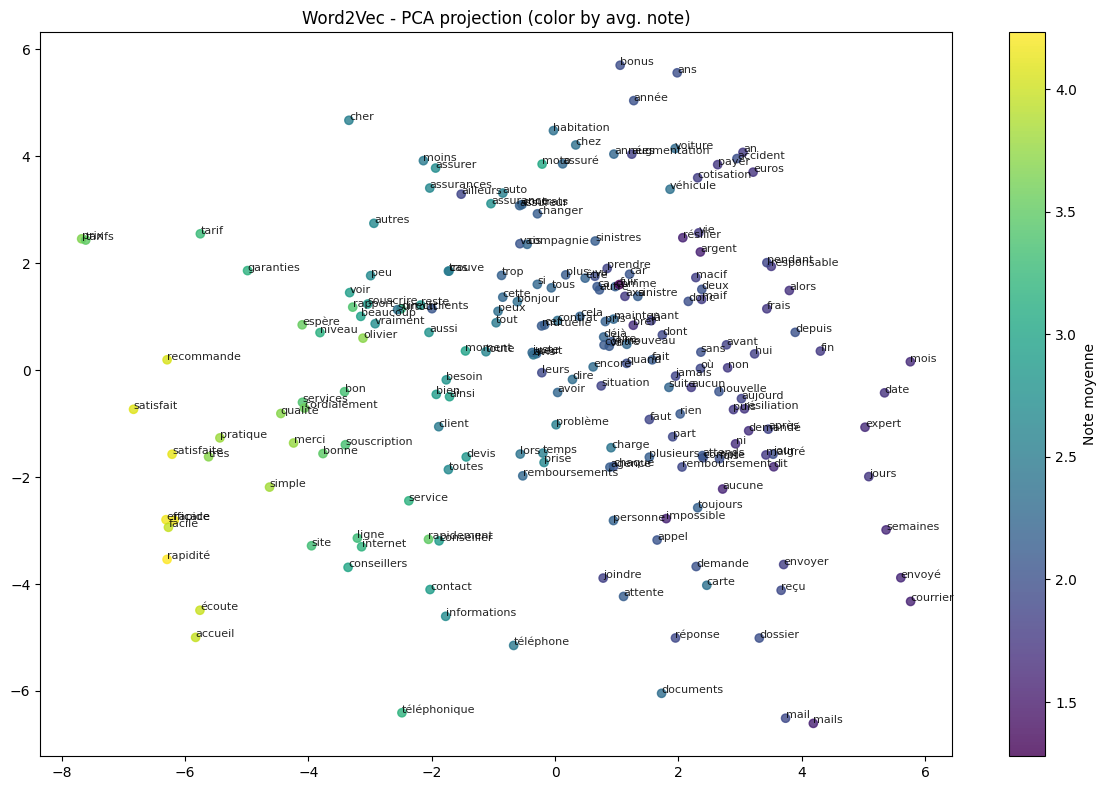
\includegraphics[width=\linewidth]{Word2Vec_2D_PCA.png}
    \caption{Word2Vec PCA (2D).}
  \end{subfigure}\hfill
  \begin{subfigure}{0.48\textwidth}
    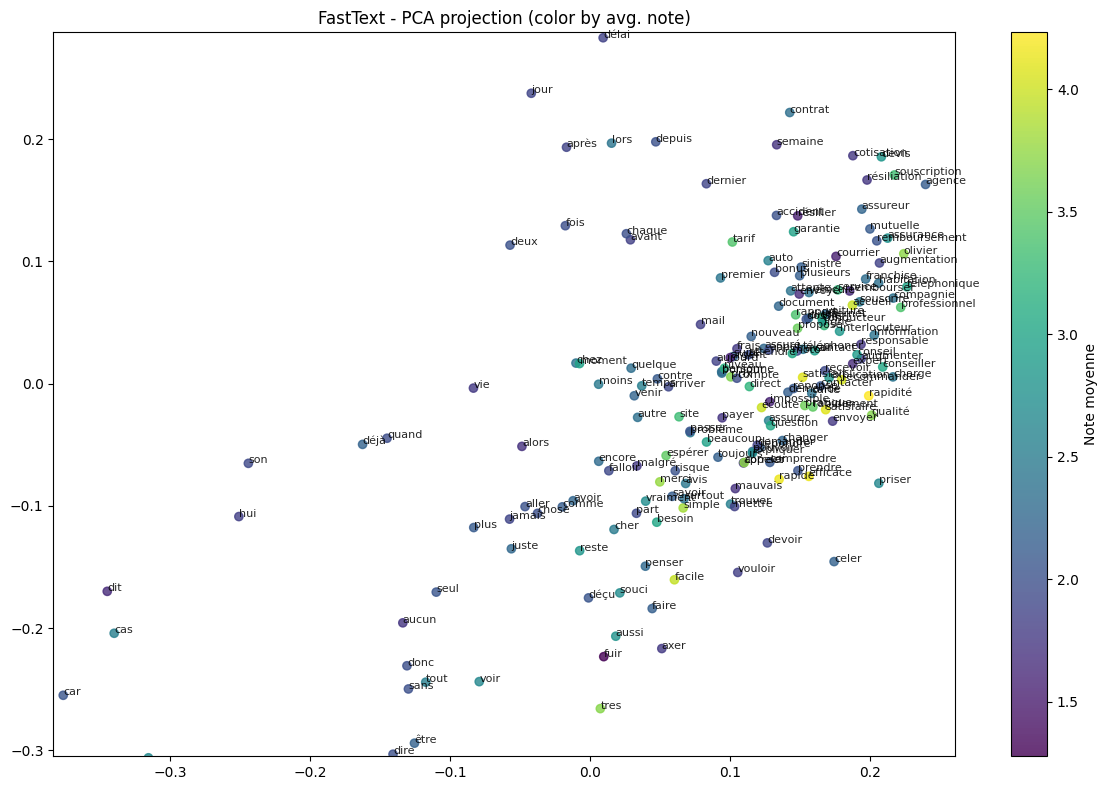
\includegraphics[width=\linewidth]{FastText _PCA_2Dprojection.png}
    \caption{FastText PCA (2D), same sampling logic.}
  \end{subfigure}
  \caption{PCA projections of embedding spaces (color encodes average rating where available).}
  \label{fig:w2vft}
\end{figure}

\begin{figure}[htbp]
  \centering
  \begin{subfigure}{0.48\textwidth}
    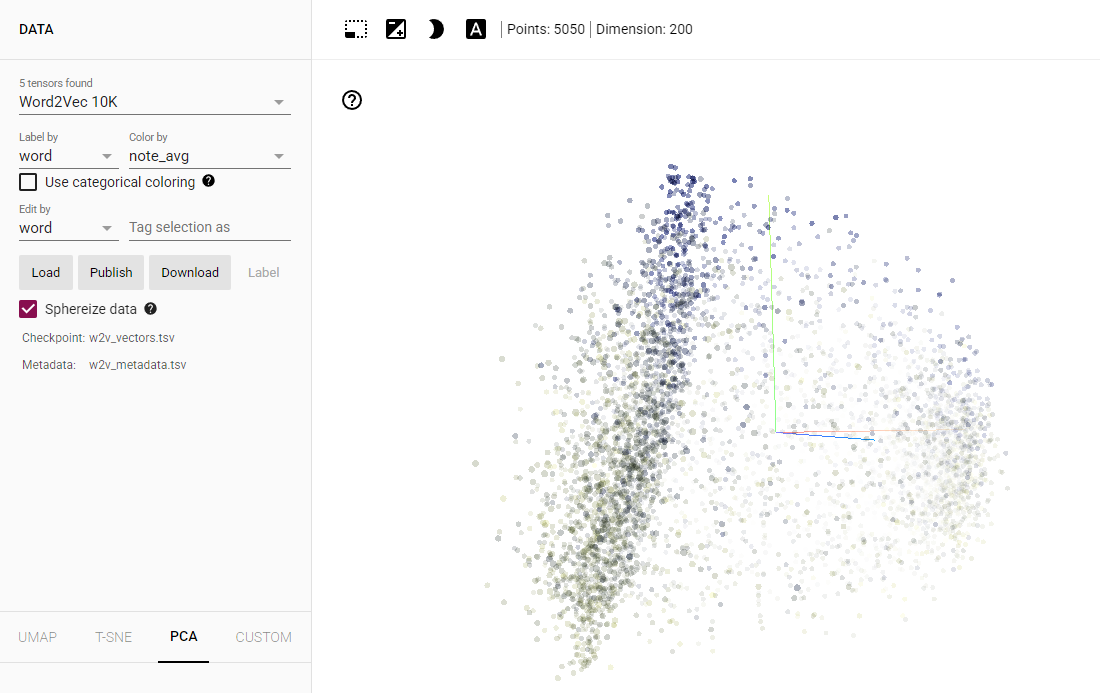
\includegraphics[width=\linewidth]{w2w_3D_projector_1.png}
    \caption{TensorBoard-style 3D view (Word2Vec export).}
  \end{subfigure}\hfill
  \begin{subfigure}{0.48\textwidth}
    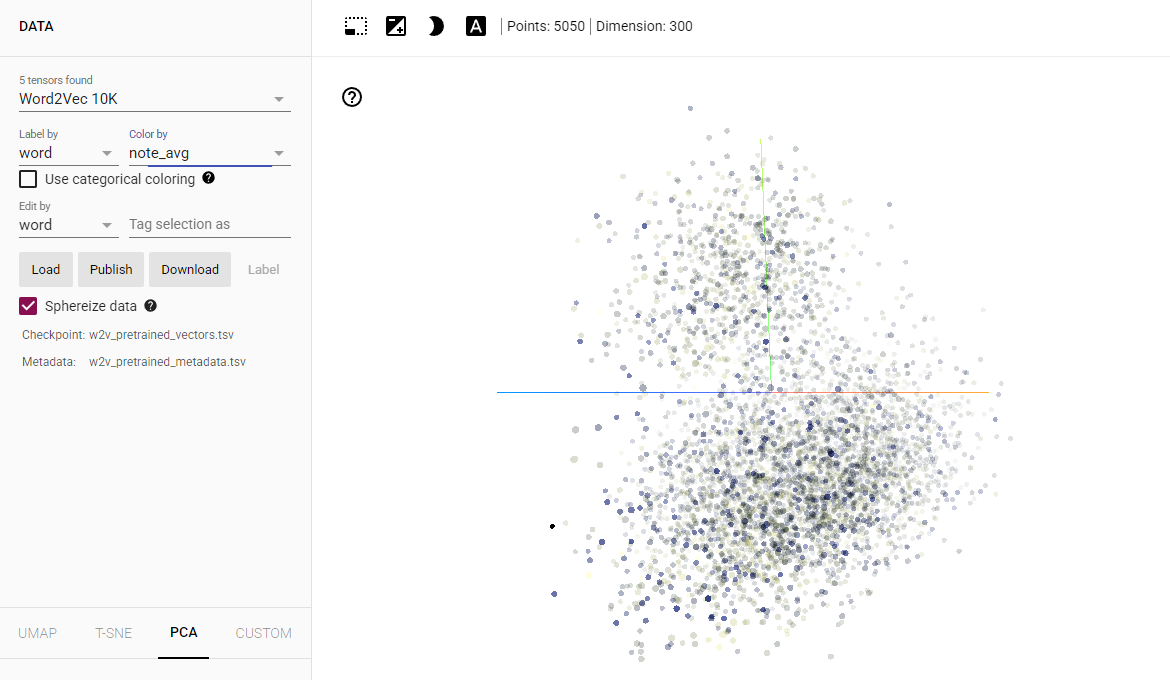
\includegraphics[width=\linewidth]{FastText _3D.png}
    \caption{3D projection for FastText vectors.}
  \end{subfigure}
  \caption{Three-dimensional embedding visualizations for exploration.}
  \label{fig:emb3d}
\end{figure}

\section{Qualitative embedding figures analysis}
\label{sec:qual-emb}
Thematic probes in the trained Word2Vec space show that lexicon associated with opposite customer experiences tends to occupy distant regions of the vector space. For example, \textit{refus} (denial, rejection) anchors a neighborhood of terms linked to dissatisfaction and conflict, whereas \textit{amabilité} (kindness, courtesy) sits among vocabulary typical of positive service descriptions. In the TensorBoard views, these seeds and their neighbors therefore appear as two poles: negatively connoted words cluster away from positively connoted ones, which is consistent with distributional semantics capturing sentiment and interaction quality from co-occurrence in reviews.

This separation aligns with the global structure visible in the PCA and 3D panels above (Figures~\ref{fig:w2vft} and~\ref{fig:emb3d}), but \textbf{much more clearly for domain-trained Word2Vec than for pretrained FastText}. In both two-dimensional PCA plots and three-dimensional projector renderings, points are coloured by the average star rating of reviews in which each word appears (the \texttt{viridis} scale). For \textbf{Word2Vec}, one observes a clear stratification: high-rated contexts tend toward one end of the palette (bluer tones), while low-rated contexts shift toward the other (yellower tones), so the delineation by score is \textbf{visually strong and interpretable}. For \textbf{FastText} (Common Crawl French, not fine-tuned on reviews), the same colouring yields a \textbf{far muddier} picture: blue and yellow points intermingle, and the boundary between score-induced regions is \textbf{barely visible} compared with Word2Vec. That gap is expected, crawl embeddings optimise general French usage, not insurer-specific sentiment, whereas Word2Vec was trained directly on this corpus, so co-occurrence with satisfied versus dissatisfied language is baked into the geometry. The cloud is never perfectly linear even for Word2Vec, polysemy and mixed opinions blur boundaries, but the rating-graded manifold is unmistakable there, and only weakly echoed in the static FastText views, which is why thematic probes such as \textit{refus} versus \textit{amabilité} read most clearly against the Word2Vec background.

\begin{figure}[htbp]
  \centering
  \begin{subfigure}{0.48\textwidth}
    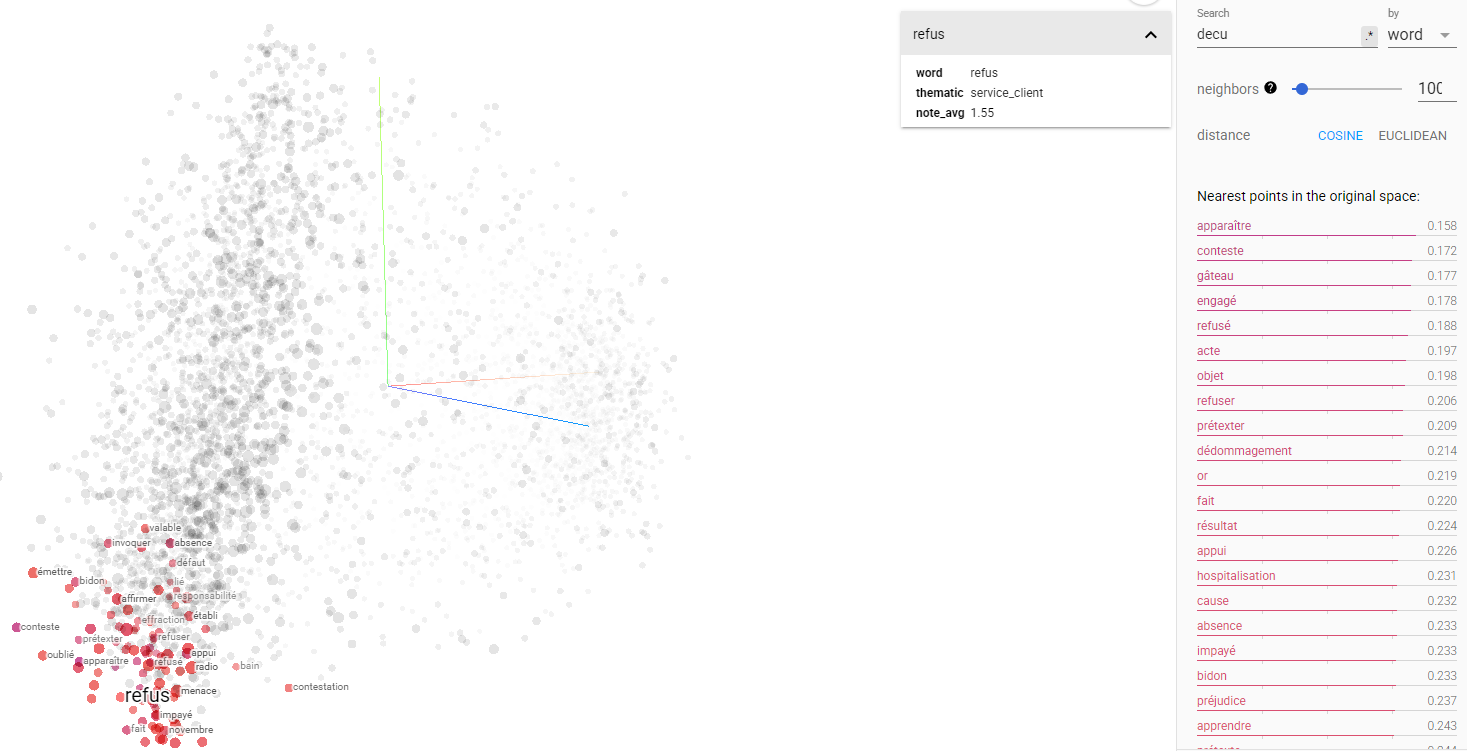
\includegraphics[width=\linewidth]{w2w_3D_refus.png}
    \caption{Neighborhood probe: \textit{refus}.}
  \end{subfigure}\hfill
  \begin{subfigure}{0.48\textwidth}
    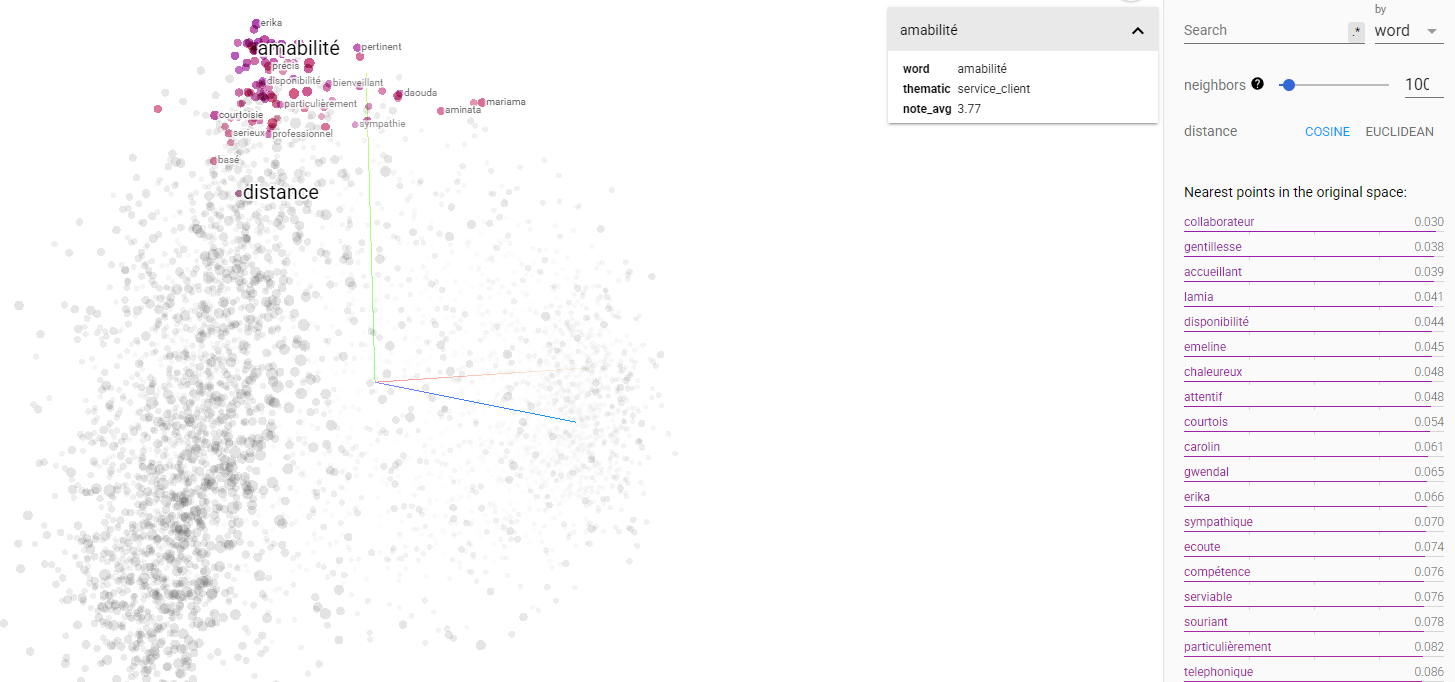
\includegraphics[width=\linewidth]{w2w_3D_amabilité.png}
    \caption{Neighborhood probe: \textit{amabilité}.}
  \end{subfigure}
  \caption{Word2Vec embedding projector views for thematic interpretation.}
  \label{fig:qual-probes}
\end{figure}

\FloatBarrier

\section{LDA topic exploration}
Latent Dirichlet Allocation used bigram documents, a dictionary/TF-IDF corpus, and \texttt{LdaMulticore} with \texttt{alpha='asymmetric'} and \texttt{eta='auto'}. The number of topics $k$ was selected from $\{4,6,8,10,12\}$ by maximizing the $c_v$ coherence score from Gensim's \texttt{CoherenceModel}, which balances interpretability against granularity. TF-IDF weighting reduces the dominance of ultra-frequent terms before topic induction.

\section{Supervised thematic classification}
Thematic labels for training come from a deterministic keyword and Word2Vec-augmented detector applied in the notebook, yielding classes such as \texttt{service\_client}, \texttt{prix}, \texttt{sinistres}, and \texttt{remboursements}.

\textbf{TF-IDF + logistic regression:} \texttt{TfidfVectorizer(max\_features=5000, ngram\_range=(1,2))} captures unigrams and bigrams within a controlled vocabulary; \texttt{LogisticRegression(max\_iter=500, random\_seed=42)} provides a strong linear baseline with calibrated probabilities under mild sparsity; see the vectorizer documentation~\cite{ref:sklearn-tfidf}.

\textbf{Fine-tuned DistilBERT:} The base checkpoint \texttt{distilbert-base-multilingual-cased}~\cite{ref:distilbert} matches the French (and mixed) text while remaining lighter than full BERT. Training uses the Hugging Face \texttt{Trainer} API~\cite{ref:hf-trainer} with \texttt{MAX\_LEN=128} (sufficient for lemmatized reviews and standard for DistilBERT fine-tunes), learning rate $2\times 10^{-5}$, batch sizes 16 (train) and 32 (eval), two epochs, evaluation each epoch, no checkpoint saving to disk during training, mixed precision when CUDA is available, and a stratified 80/20 split. These choices follow widespread practice for sentence classification on transformer encoders~\cite{ref:distilbert}. The fine-tuned weights are saved under \texttt{artifacts/distilbert\_thematic/} for the application.

\section{Streamlit application architecture}
Figure~\ref{fig:arch} sketches the main flows. The \textbf{single-review} tab runs preprocessing, DistilBERT thematic probabilities, a French summarizer, a multilingual sentiment head, and similar-review retrieval. The \textbf{RAG} tab embeds chunked reviews and calls a local LLM for grounded answers.

\begin{figure}[htbp]
\centering
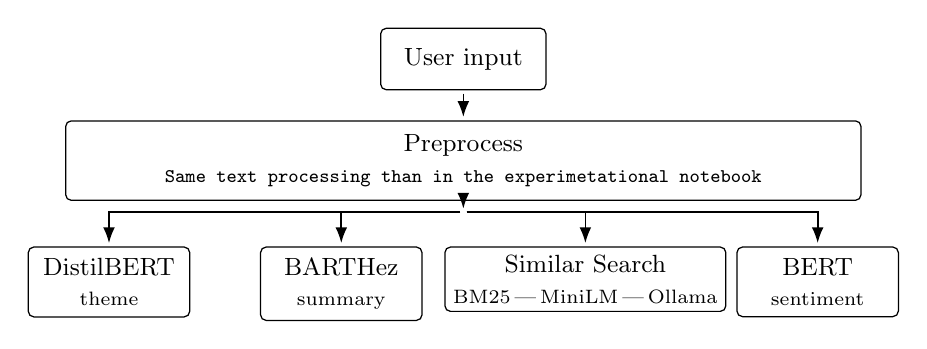
\begin{tikzpicture}[
  font=\small,
  node distance=0.42cm,
  box/.style={
    draw,
    rounded corners=2pt,
    align=center,
    inner sep=5pt,
    minimum height=0.78cm,
    line width=0.45pt,
  },
  arr/.style={
    -{Latex[length=2mm,width=1.5mm]},
    semithick,
    shorten >=1.2pt,
    shorten <=1.2pt,
  },
]
  % Top: input, then wide preprocess (matches widened bottom row)
  \node[box, minimum width=2.1cm] (inp) {User input};
  \node[box, minimum width=10.1cm, below=0.38cm of inp] (prep)
    {Preprocess\\\texttt{\scriptsize Same text processing than in the experimetational notebook}};
  % Junction just under preprocess (orthogonal fan-out, no edge crossing boxes)
  \coordinate (hub) at ($(prep.south)+(0,-0.14)$);
  \draw[arr] (inp) -- (prep);
  \draw[arr] (prep.south) -- (hub);
  % Bottom row: larger horizontal gaps (centres at ±4.5 / ±1.55); similar box kept narrow (short label)
  \node[box, minimum width=2.05cm, inner sep=4pt, anchor=north] (db)   at (-4.5,-2.38) {DistilBERT\\\scriptsize theme};
  \node[box, minimum width=2.05cm, inner sep=4pt, anchor=north] (sum)  at (-1.55,-2.38) {BARTHez\\\scriptsize summary};
  \node[box, minimum width=1.68cm, inner sep=3pt, anchor=north] (sim)  at ( 1.55,-2.38)
    {Similar Search\\\scriptsize BM25\,|\,MiniLM\,|\,Ollama};
  \node[box, minimum width=2.05cm, inner sep=4pt, anchor=north] (sent) at ( 4.5,-2.38) {BERT\\\scriptsize sentiment};
  \foreach \t in {db,sum,sim,sent} {\draw[arr] (hub) -| (\t.north);}
\end{tikzpicture}
\caption{Simplified single-review analysis pipeline in the Streamlit app.}
\label{fig:arch}
\end{figure}

\textbf{Summarization:} uses \texttt{moussaKam/barthez-orangesum-abstract}~\cite{ref:barthez} (French BART-style model). Generation uses \texttt{do\_sample=False}, dynamic \texttt{max\_length} and \texttt{min\_length} from review length, truncation, and a minimum word threshold so very short texts skip summarization.

\textbf{Sentiment:} uses \texttt{nlptown/bert-base-multilingual-uncased-sentiment}~\cite{ref:sentiment-bert} (five-star heads); star predictions are mapped to coarse polarity for display.

\textbf{Similar reviews:} \texttt{rank\_bm25} implements Okapi BM25~\cite{ref:bm25} over French-tokenized corpus rows (default cap 4{,}000 rows for latency). The bi-encoder is \texttt{sentence-transformers/all-MiniLM-L6-v2}~\cite{ref:minilm-l6} (384-d, efficient English-oriented sentence embeddings; acceptable here for shared insurance vocabulary). Pipeline: top 50 BM25 $\rightarrow$ top 25 by cosine similarity $\rightarrow$ top 10 pool $\rightarrow$ optional Ollama rerank with \texttt{llama3.2}~\cite{ref:ollama-llama}, temperature 0.1, short \texttt{num\_predict} for a numeric similarity score, yielding five final hits.

\textbf{RAG:} Chunks default to 90 words with 20-word overlap. Embeddings use \path{paraphrase-multilingual-MiniLM-L12-v2}~\cite{ref:paraphrase-l12} (multilingual semantic search, 384-d). Retrieval is cosine similarity on L2-normalized vectors; generation uses Ollama \texttt{llama3.2}~\cite{ref:ollama-llama} with temperature 0.3 and bounded context in the user prompt. Index build parameters are fingerprinted so stale indices are detectable when CSV or hyperparameters change.

\textbf{Demonstration.} This written overview cannot capture every interaction detail of the Streamlit interface (tab layout, index build button, insurer filter, error states when Ollama is offline, etc.). A separate \emph{explanatory video} accompanies the project: it walks through the application end-to-end, demonstrates the RAG tab with sample questions, and shows the single-review pipeline on real pasted text. Refer to that recording for a precise, step-by-step view of how the app is operated and what to expect on screen.

\section{Limitations and conclusion}
The pipeline mixes research prototypes (partial spell-check and translation coverage, capped similar-review corpus, RAG document limits) with solid core modeling (stratified splits, coherence-driven LDA, DistilBERT fine-tuning). Production use would require full-data cleaning, systematic evaluation on held-out temporal splits, monitoring of Ollama latency and failures, and privacy review of third-party model endpoints if any were introduced. Overall, the project demonstrates a coherent stack from classical NLP through transformers to retrieval-augmented generation, with explicit hyperparameters and traceable model cards.


\phantomsection
\begin{thebibliography}{99}

\bibitem{ref:gensim-w2v}
R.~Rehurek, \emph{Gensim: Word2Vec model documentation.}
\url{https://radimrehurek.com/gensim/models/word2vec.html}

\bibitem{ref:fasttext-vec}
Facebook Research, \emph{FastText: Pretrained vectors for 157 languages.}
\url{https://fasttext.cc/docs/en/pretrained-vectors.html}

\bibitem{ref:sklearn-tfidf}
scikit-learn developers, \emph{TfidfVectorizer.}
\url{https://scikit-learn.org/stable/modules/generated/sklearn.feature_extraction.text.TfidfVectorizer.html}

\bibitem{ref:distilbert}
Hugging Face, \emph{distilbert-base-multilingual-cased} model card.
\url{https://huggingface.co/distilbert-base-multilingual-cased}

\bibitem{ref:hf-trainer}
Hugging Face, \emph{Transformers: Trainer API.}
\url{https://huggingface.co/docs/transformers/main_classes/trainer}

\bibitem{ref:barthez}
Moussa Kamalis et al., \emph{moussaKam/barthez-orangesum-abstract.}
\url{https://huggingface.co/moussaKam/barthez-orangesum-abstract}

\bibitem{ref:sentiment-bert}
nlptown, \emph{bert-base-multilingual-uncased-sentiment.}
\url{https://huggingface.co/nlptown/bert-base-multilingual-uncased-sentiment}

\bibitem{ref:bm25}
PyPI, \emph{rank-bm25: BM25 ranking function implementation.}
\url{https://pypi.org/project/rank-bm25/}

\bibitem{ref:minilm-l6}
sentence-transformers, \emph{all-MiniLM-L6-v2.}
\url{https://huggingface.co/sentence-transformers/all-MiniLM-L6-v2}

\bibitem{ref:ollama-llama}
Ollama, \emph{Llama~3.2} library page.
\url{https://ollama.com/library/llama3.2}

\bibitem{ref:paraphrase-l12}
sentence-transformers, \emph{paraphrase-multilingual-MiniLM-L12-v2.}
\url{https://huggingface.co/sentence-transformers/paraphrase-multilingual-MiniLM-L12-v2}

\end{thebibliography}

\end{document}
